\section{Signal Acquisition} 
\label{chap:SignalAcquisition}
All autonomous vehicles must have a sufficient knowledge of the surrounding environment and obtain accurate location information. For this purpose different sensors need to be adopted on a single vehicle, as a matter of fact different sensor have different limitations which can be overcome through sensor fusion. This approach is able to compensate the limitations of one sensor with the strengths of another.
%%%%%%%%%%%%%%%%%%%%%%%%%%%%%%%%%%%%%%%%%%
\subsection{Sensors used in obstacle avoidance}
When dealing with autonomous driving, three are the core functions of interest: 
\begin{itemize}
    \item perception: visual perception (e.g., camera) and radar perception (e.g., LIDAR);
    \item planning: GPS, Inertial Navigation System (INS), and HD Maps;
    \item control: image identification, deep learning and artificial neural networks.
\end{itemize}

\subsection{Perception: what a self-driving car sees}
The three primary autonomous vehicle sensors for perception are camera, radar and lidar. Working together, they provide the car visuals of its surroundings and help it to detect the speed and distance of nearby objects, as well as their three-dimensional shape. \cite{NVIDIA}

\subsubsection{Camera} 
Cameras are the main type of sensors for creating a visual representation of the surrounding world, as a matter of fact autonomous vehicles rely on cameras placed on every side to stitch together a 360 degrees view of their environment.
Though providing very accurate images up to 80 meters, cameras have limitations:
\begin{itemize}
    \item the distance from target objects needs to be calculated in order to know exactly where they are;
    \item mechanical issues: mounting multiple cameras as well as keeping them clean;
    \item issues related to low visibility conditions (e.g., rain, fog, nighttime);
    \item heavy graphic processing needed.
\end{itemize}

\subsubsection{Radar} \label{radar}
Radars can overcome cameras limitations in low visibility scenarios and improve object detection.
The working principle of radars is based on radio pulses emitted by a source. Once these pulses hit an object they travel back to the sensor providing information about its speed and location. 
The maximum distance range for radar-based sensors is 250 meters for Long-Range Radars, 100 meters for Medium-Range Radars and 30 meters for Short-Range Radar.

\subsubsection{Lidar}
The name LiDAR stands for Light Detection and Ranging and its working principle is analogous to the radar's (Sub-section \ref{radar}) but using a different part of the electro-magnetic spectrum. Radars use radio waves or microwaves while lidars use light near the visible spectrum.
This type of sensors make it possible for an autonomous car to create a 3D point cloud map and they provide shape and depth of the surroundings and its actors.

\subsection{Planning: know where a self-driving car is going}

\textit{``As the core of the planning layer, localization and navigation technologies including GPS, INS, and HD maps aim to assist self-driving cars in planning routes and navigating in real time."} \cite{luo2019localization}

\vspace{2mm}

The above-mentioned technologies which have to be always active, allow the vehicle to go from point A to point B following the optimal route, and must re-compute in real-time the path if the optimal one has any unexpected diversions using a well tuned controller.

\subsubsection{GPS}
GPS stands for Global Positioning System. A GPS receiver is able to compute the current position of the vehicle together with the current time, acquiring and analysing signals received from at least four of the constellation of over 60 low-orbit satellites. 
The accuracy on the position information is 1 meter.

\subsubsection{INS}
INS stands for Inertial Navigation System and allows the accurate sensing of high-precision 3D position, velocity, and attitude information of the car via the inertial measurement unit (IMU).
It can make up for the deficiency of GPS localization, which is not real-time enough.

\subsubsection{HD Maps}
HD Maps are crucial when it comes to Self-Driving Vehicles, these high-definition 3D maps are highly accurate and contain details not normally present on traditional maps. Such maps can be precise at a centimetre level.
HD Maps consist of two map layers: static and dynamic HD Map.
The former is usually collected in advance and contains lane models, road information, and road attributes while the latter, stored on a cloud platform, contains real-time traffic information. Moreover, dynamic HD Maps can be updated in real-time through information collected from vehicles and infrastructures on the cloud.

\subsection{Our Assumptions}

Our model is based on several assumptions regarding data acquisition from the sensors and how these data are translated into useful information. Below the list of assumptions we have made:
\begin{itemize}
    \item we suppose no error in the information collected from the sensors;
    \item our car knows all the information related to the road model, such as lane width and number of lanes by acquiring them from cameras installed on the vehicle and HD Maps;
    \item the vehicle knows its position in the XY reference frame, through the use of GPS and INS;
    \item the route planning done by our controller exploits the latitude and longitude information to plan out a complete route based on the HD Maps, GPS, and INS. Moreover, while driving, the car also compares the HD maps with the perception information from sensors to get changing environment information for dynamically planning routes and making decisions;
    \item we suppose to have both a Long-Range Radar and Lidar mounted on the vehicle, hence to be able to detect obstacles in the range of 100 meters;
\end{itemize}

Though we include all the above information on the MATLAB code, we suppose to collect them using sensors, as previously described.







%%%%%%%%%%%%%%%%%%%%%%%%%%%%%%%%%%%%%%%%%%

\subsection{Reference trajectory}
After implementing the vehicle model and keeping in mind the assumptions made above, we have generated and imposed a reference trajectory to the vehicle in order to have a path to follow during the development and the testing phases.
To do so, we have taken the desired scenario from a real map using the open source website \href{https://www.openstreetmap.org}{\textit{OpenStreetMap}}\cite{OpenStreetMap} (Figure \ref{fig:OpenStreetMap}).
The website allows the user to export any route as a \textit{.osm} file containing the global coordinates of the area together with some useful metadata such as street name, number of lanes, speed limits, etc.

\begin{figure}[H]
    \centering
    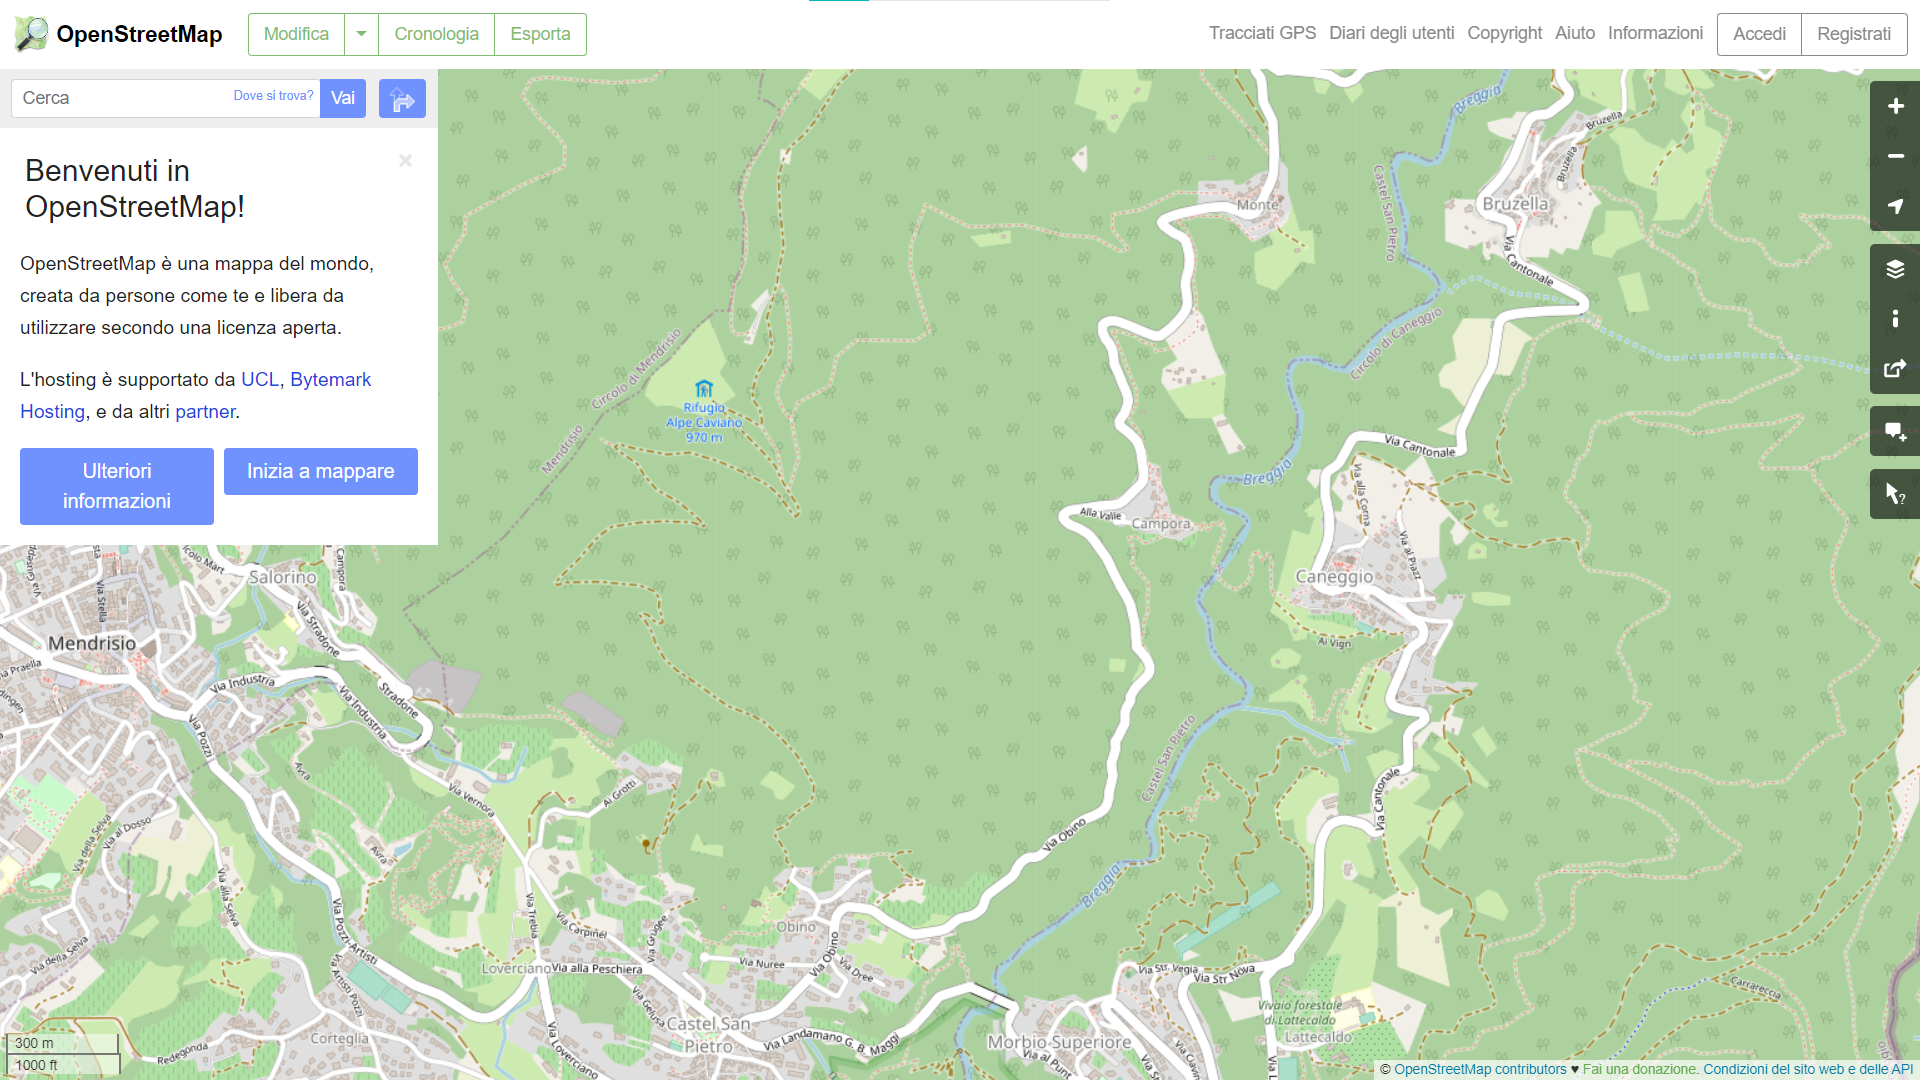
\includegraphics[width=1\textwidth]{Figures/OpenStreetMap.png}
    \caption{Selecting the area of interest in \textit{OpenStreetMap}}
      \label{fig:OpenStreetMap}
\end{figure}

Next, we have imported the \textit{.osm} file in MATLAB exploiting the \textit{Driving Scenario Designer} tool (Figure \ref{fig:DrivingScenarioTool}) provided by MATLAB itself. The Driving Scenario Designer tool splits the whole selected route in as many pieces as the number of different streets names present. Then, the user can select only the pieces of road he/she is interested in and export its waypoints in a \textit{.mat} file.

\begin{figure}[H]
    \centering
    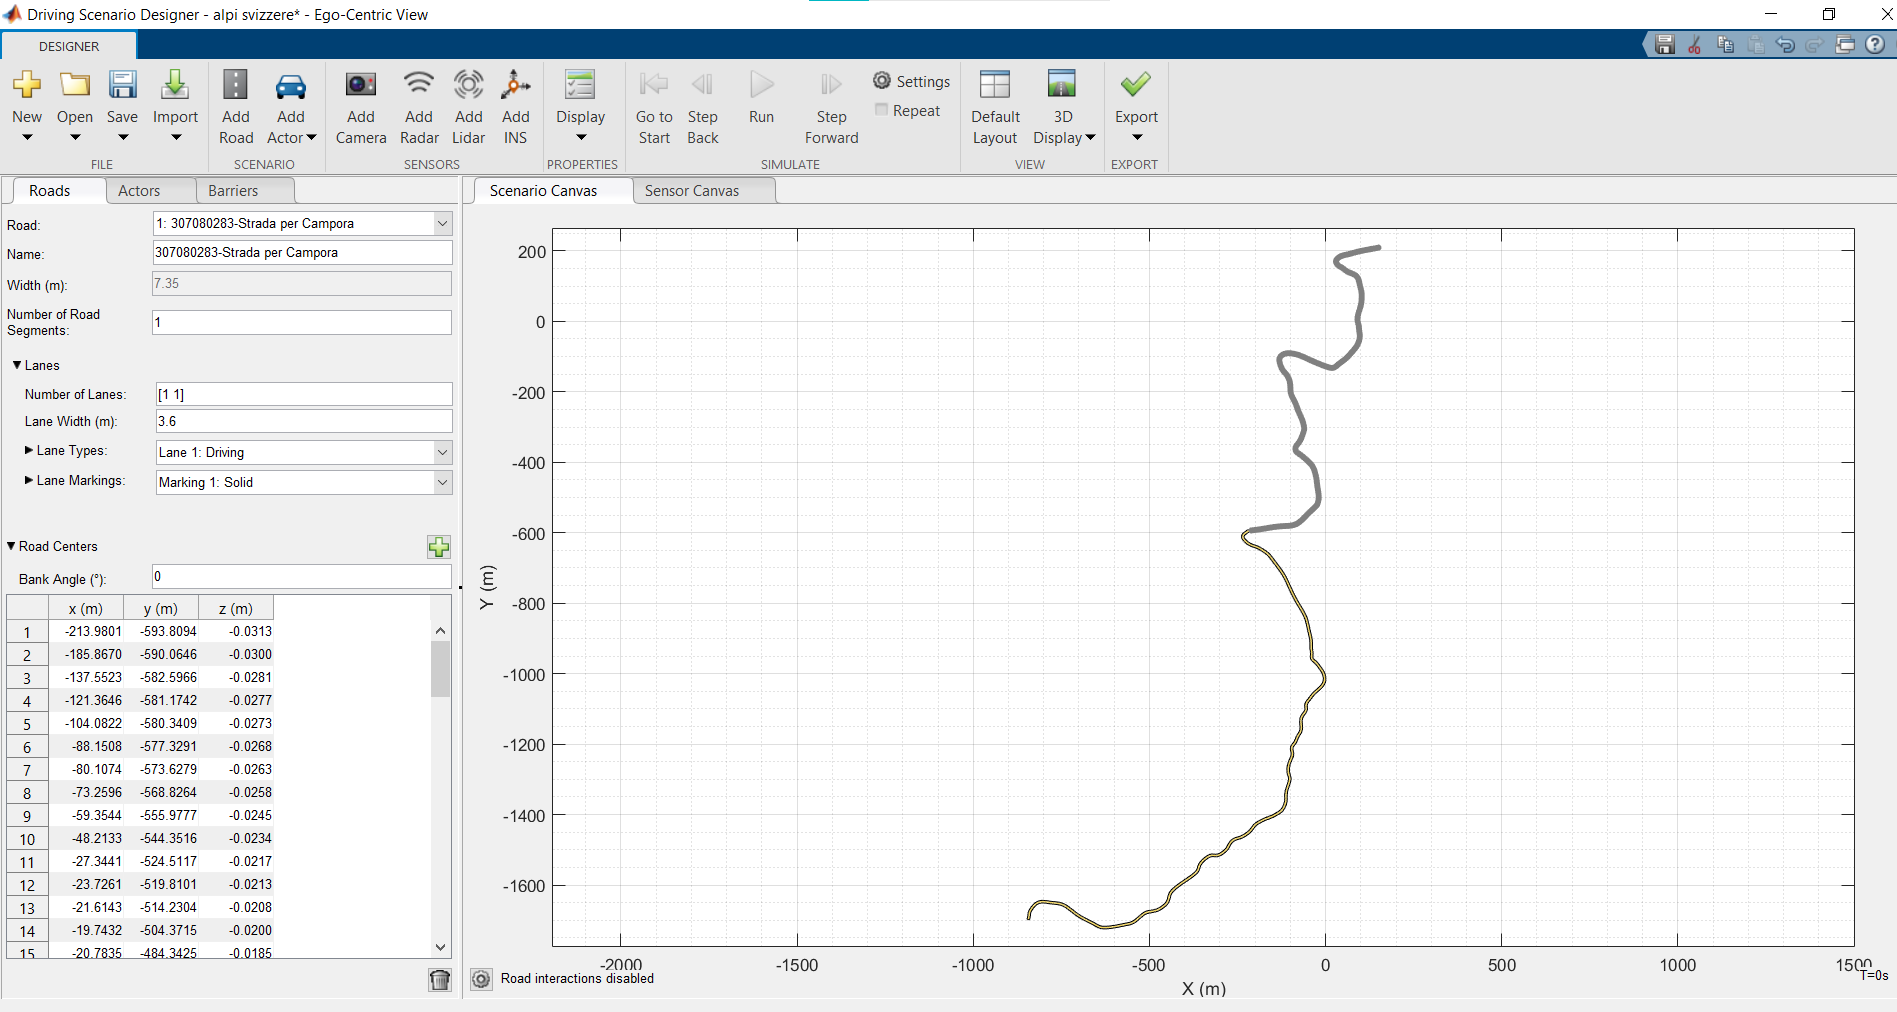
\includegraphics[width=1\textwidth]{Figures/DrivingScenarioTool.png}
    \caption{Importing maps on MATLAB using \textit{Driver Scenario Designer}}
      \label{fig:DrivingScenarioTool}
\end{figure}

Afterwards, the \textit{.mat} file is used to generate the corresponding map in the \textit{XY} reference frame.
Since the thus generated map is composed by an insufficient number of waypoints for our applications, we have decided to create a function able to do an up-sample of the map because a higher density of points on it optimizes the path following algorithm. The up-sampling function interpolates linearly the original map with a fixed step depending on the reference speed and the sampling time selected for the controller. \\
It is worth mentioning, as shown in Figure \ref{fig:UpSample}, that the up-sampled path (in orange) and the original waypoints (in blue) slightly deviate in some sections of the route due to the smoothing applied in order to obtain a more gentle trajectory.

\begin{figure}[H]
    \centering
    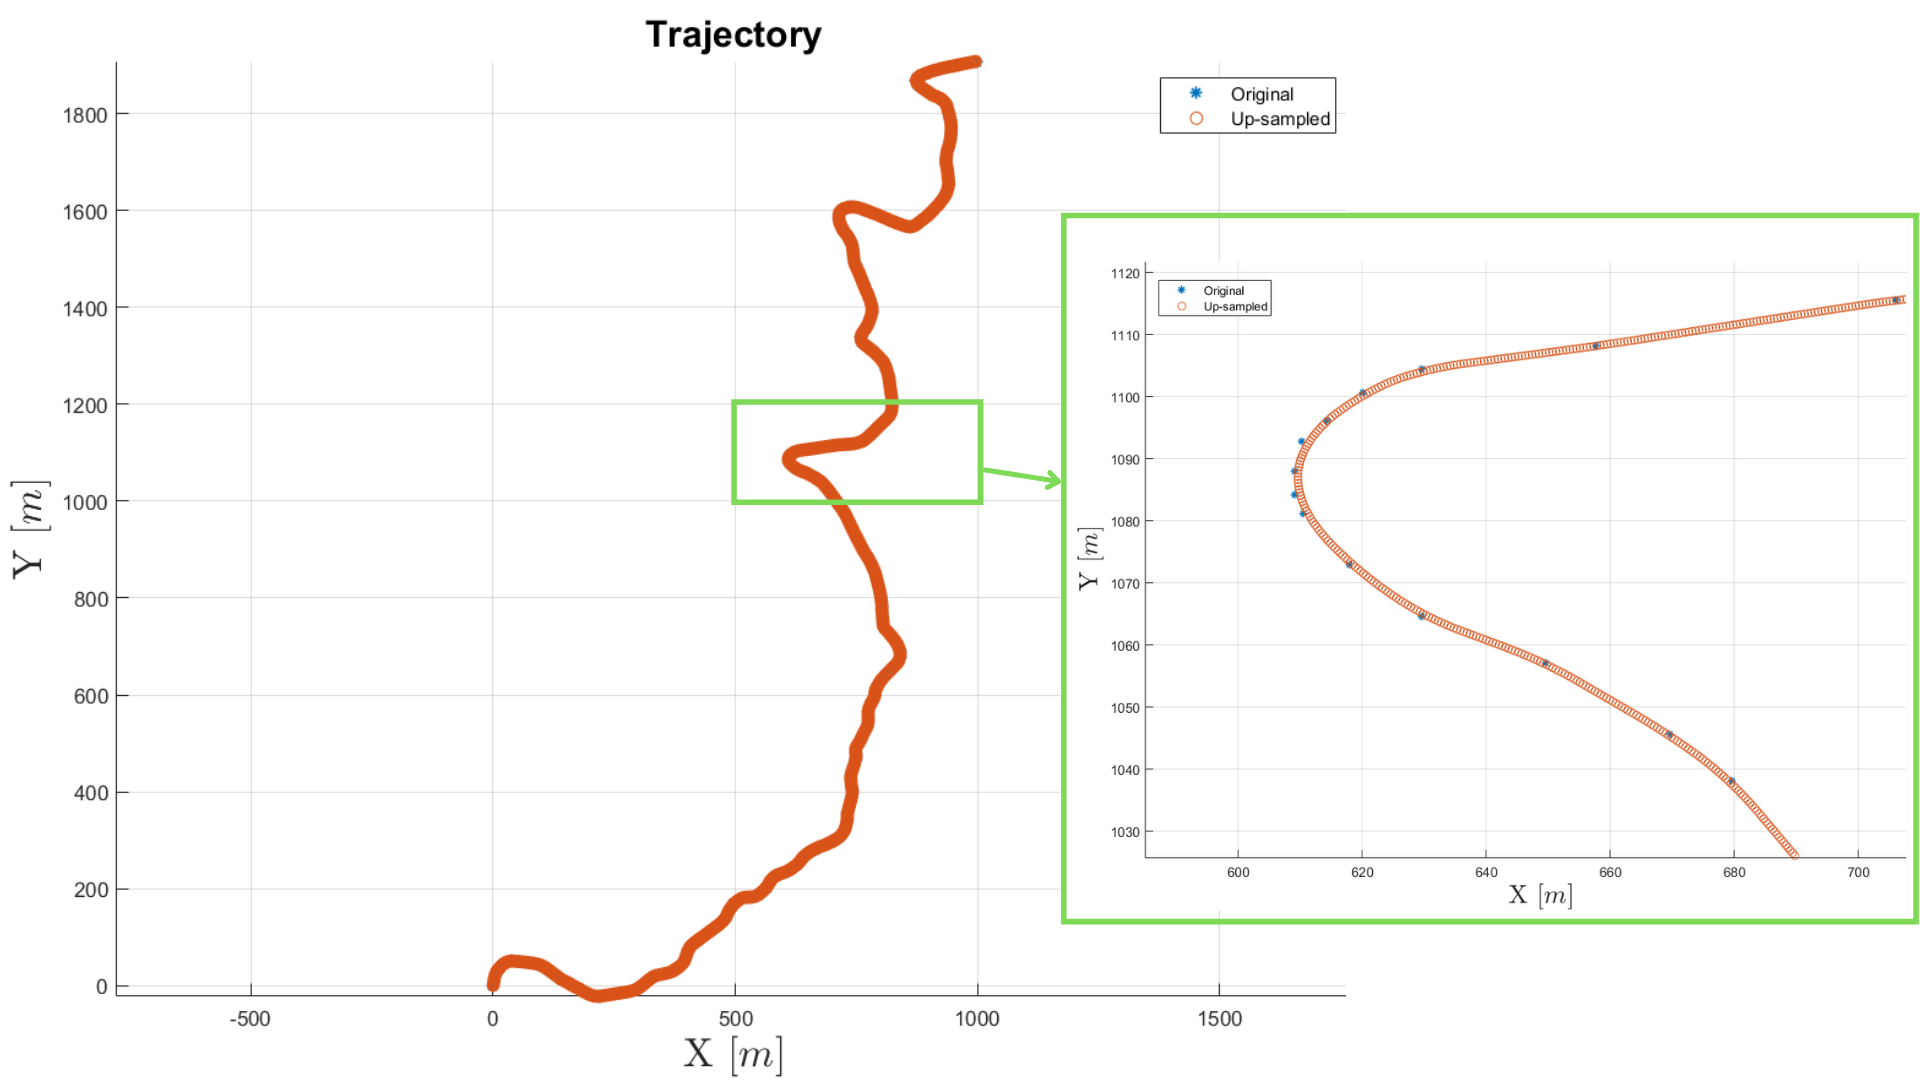
\includegraphics[width=1\textwidth]{Figures/UpSample.png}
    \caption{Comparison between original and up-sampled path}
      \label{fig:UpSample}
\end{figure}

%%%%%%%%%%%%%%%%%%%%%%%%%%%%%%%%%%%%%%%%%%%%%%%%

%\subsection{Obstacles acquisition}